% !TEX encoding = UTF-8
% !TEX program = xelatex
\documentclass[12pt,a4paper]{article}
\usepackage[paperwidth=210mm, paperheight=297mm, left=0.75in, right=0.75in, bottom=1in, top=1in]{geometry}
\usepackage{polyglossia}
\setdefaultlanguage[babelshorthands]{italian}
\usepackage{fontspec}
\usepackage{graphicx}
\usepackage{blindtext}
\usepackage{wrapfig}

\frenchspacing
\makeindex

\begin{document}
\title{\vspace{-70pt}Fermi (Gamma-ray Large Area Space Telescope)}
\author{Paolo Piola}
\date{}
\maketitle
\pagestyle{empty}
\thispagestyle{empty}

\section*{Storia}
\label{storia}
\begin{wrapfigure}{r}{0.35\textwidth}
  \vspace{-10pt}
  \begin{center}
    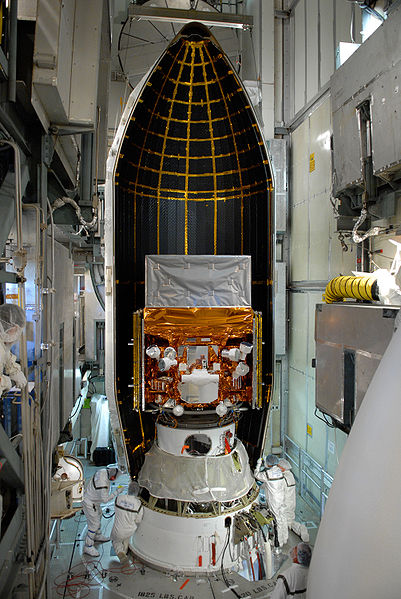
\includegraphics[width=0.30\textwidth]{satellite}
  \end{center}
  \vspace{-20pt}
\end{wrapfigure}
Il \emph{Telescopio Spaziale di Grande Area per Raggi Gamma},in seguito ribattezzato Fermi il 28 agosto 2008 in onore di Enrico Fermi,è stato lanciato in orbita l'11 giugno 2008. Esperimento approvato dalla NASA nel 2001 ha la finalità di \emph{studiare} la radiazione elettromagnetica emessa dai corpi celesti compresa tra 8 keV e 300 GeV ovvero \emph{i raggi gamma}.

\section*{Osservazioni}
\label{osservazioni}

L'apparato comprende due strumenti scientifici:

\begin{itemize}
\item il \emph{Large Area Telescope} (LAT) sensibile alla radiazione gamma tra 20 MeV e 300 GeV.

\item il \emph{Gamma-Ray Burst Monitor} (GBM) per lo studio di radiazioni con energie relativamente più basse ovvero tra 8 keV e 40 MeV;

\end{itemize}

Il principio di funzionamento del LAT si basa sull'interazione tra raggi gamma e materia ovvero la \emph{produzione di coppie di elettroni e positroni} (antimateria). Lo strumento ha a disposizione delle torrette rilevatrici al silicio. All'interno di esse vi sono delle \emph{lamine sottili di Tungsteno}. I raggi gamma a contatto con esse producono elettroni e positroni. L'energia viene rilevata da un \emph{calorimetro elettromagnetico} di Ioduro di Cesio e tramite il \emph{tracciatore al Silicio} dalle coppie elettrone-positrone si può risalire alla traiettoria del fotone incidente.

Tra il 2008 e il 2009 Fermi scopre numerose \emph{pulsar e stelle di neutroni}. Il 9 novembre 2010: Fermi rivela due gigantesche strutture che si estendono per 25 mila anni luce al di sopra e al di sotto del piano galattico. Queste due strutture, soprannominate \emph{“bolle di Fermi”}, potrebbero essere il resto di una \emph{eruzione proveniente dal centro della Galassia} alcuni milioni di anni fa. 

Il 10 gennaio 2011 Fermi rivela l’antimateria generata dai \emph{lampi di raggi gamma} (Terrestrial Gamma Ray Flashes - TGRF) \emph{generati sul nostro pianeta} dalle grandi nubi temporalesche nelle zone equatoriali.

\section*{Curiosità}
\label{curiosit}

Le osservazioni del satellite Fermi riguardo ai TGRF hanno dato una spinta verso lo studio di questo \emph{raro e misterioso fenomeno} che può addirittura costituire un serio \emph{pericolo per la navigazione area}. 


\end{document}